\documentclass[10pt,a4paper]{article}
\usepackage[margin=2cm]{geometry}
\usepackage[T1]{fontenc}
\usepackage{lmodern}
\usepackage{microtype}
\usepackage{graphicx}
\usepackage{booktabs}
\usepackage{amsmath}
\usepackage{caption}
\usepackage[hidelinks]{hyperref}
\captionsetup{font=small,labelfont=bf}
\setlength{\parskip}{3pt}

\title{Where do riders stay?\\[2pt]\large Functional neighbourhoods in New York's Citi Bike trip flows}
\author{02807 Computational Tools for Data Science, final project\\[4pt]
  % TODO: names and student numbers of all group members
  Full Name (s000000)}
\date{December 2026}

\begin{document}
\maketitle

\noindent\textbf{Summary.}
Using all 45.7 million Citi Bike trips from September 2025 to August 2026, we ask which parts of New York work as \emph{self-contained} bike-share areas, and whether these areas change over the day and week.
We build a trip graph over 2,384 stations and partition it with three graph-clustering methods: our own spectral clustering and modularity, Louvain, and \textbf{Infomap} (the map equation, \emph{not taught in the course}).
We test the partitions against a purely geographic baseline, the official neighbourhood boundaries and their own random-seed noise.
Separately, we cluster each station's 24-hour net-flow profile with k-means and Ward clustering.
The main findings are:
(i) Infomap and spectral clustering keep 10--15 percentage points more trips inside their areas than geography alone, while Louvain at high resolution does \emph{worse} than geography;
(ii) three functional areas cross borough borders;
(iii) only the weekday morning rush has its own structure, when the Upper East and West Sides join the Manhattan core;
(iv) station profiles form a continuum along one commuting axis rather than distinct types; and
(v) areas that keep trips inside are \emph{not} balanced in bikes.
Section~2 covers the data, Section~3 the methods, Section~4 the results and Section~5 the evaluation.

\section{Problem}
Bike-share operators move thousands of bikes a day by truck because stations run empty or full.
If the city splits into areas that riders rarely leave, rebalancing and planning could be organised per area.
Official neighbourhoods are drawn for administration, not for how people ride.
We therefore derive areas from behaviour, and ask whether they say more than ``nearby stations belong together'', which is the main risk of clustering a spatial network.

\section{Data and preprocessing}
\textbf{Source.} Citi Bike publishes one zip of trip CSVs per month in a public S3 bucket (\url{https://s3.amazonaws.com/tripdata}).
We downloaded the 12 NYC files for Sep 2025--Aug 2026 (8.3\,GB, 45.69\,M trips, 13 columns: ride id, bike type, start/end time, station name/id/coordinates, member type).
Station boundaries come from NYC Open Data (2020 Neighbourhood Tabulation Areas, NTAs: 262 NTAs nested in 71 community districts and 5 boroughs).

\textbf{Pipeline.} A resumable downloader checks file sizes against S3.
A converter checks every CSV header against the expected schema, writes typed Parquet with DuckDB and checks that no rows were lost.
All further processing runs in DuckDB SQL, one month at a time, so memory stays bounded on a 15\,GB laptop (about 3 minutes for the whole year).

\textbf{Cleaning.} Exploring the data revealed problems that are not in the documentation (Table~\ref{tab:clean}).
\emph{Station ids} like \texttt{5980.10} sometimes appear as \texttt{5980.1} (a float conversion upstream) or with a trailing underscore.
Normalising them merges, for example, 2,474 raw ids into 2,390 stations in August 2026 alone.
Six stations were renumbered without moving and are mapped onto their newest id.
\emph{Non-NYC and operator stations}: Jersey City/Hoboken (\texttt{JC*}, \texttt{HB*}) and depots (\texttt{SYS*}, and a charging depot hidden behind the id \texttt{1234.56}).
\emph{Overlapping files}: the April and May zips both contain the trips that span midnight on 30 April.
\emph{Clock change}: timestamps carry no time zone, so trips during the November daylight-saving change get negative durations.
Coordinates turned out to be station positions, not GPS, so they are reliable.
Each trip is assigned the first rule it fails, so the table adds up to the raw total.

\begin{table}[h]\centering\small
\caption{Cleaning waterfall over the 12 months (rules applied in this order).}\label{tab:clean}
\begin{tabular}{lrr}\toprule
Outcome & Trips & \% \\\midrule
kept & 45,488,697 & 99.56\\
no start/end station (e-bike left outside a dock) & 153,577 & 0.34\\
longer than 3\,h (bike not docked) & 30,180 & 0.07\\
non-NYC or operator station & 14,346 & 0.03\\
outside window / negative duration (DST) / duplicate / $>$35\,km/h / $<$60\,s & 1,897 & 0.00\\\bottomrule
\end{tabular}
\end{table}

\section{Methods}
\textbf{Graph.} Nodes are the 2,384 stations with at least one trip per active day (all stations pass).
Edge weights $W_{ij}$ count trips from $i$ to $j$, without round trips.
We build one graph for the whole year and one per time slice by start time (weekday 6--10, 10--16, 16--20, 20--6, and weekend including holidays).
The graph is dense (28\% of all pairs are linked) but the weights are very skewed (median 4 trips a year, 99th percentile 397).
Louvain, spectral clustering and modularity require an undirected graph, so they use $A=W+W^\top$.

\textbf{Course methods (graph clustering).} We implemented \emph{modularity} with a resolution parameter using sparse matrices; it matches igraph to $10^{-12}$.
We implemented \emph{spectral clustering} (Ng--Jordan--Weiss on $D^{-1/2}AD^{-1/2}$), checked on a planted-partition graph (ARI 0.94).
\emph{Louvain} comes from igraph.

\textbf{Non-course method: Infomap (the map equation).}
Modularity asks whether communities have more internal weight than a random graph with the same degrees would.
Infomap asks a different question: how cheaply can we \emph{describe the path of a random walker} on the directed, weighted graph?
It uses a two-level code: one codebook names the module the walker enters, and one codebook per module names the steps inside it.
If the walker rarely leaves a module, module names are rarely needed and the description is short.
The minimum description length $L(M)=q\,H(\mathcal{Q})+\sum_m p_m H(\mathcal{P}_m)$, where $q$ is the rate of switching modules and $p_m$ the rate of use of module $m$'s codebook, therefore picks out areas that flow stays in.
That is exactly our definition of a self-contained area.
Unlike Louvain and spectral clustering, Infomap also uses \emph{trip direction}.
The \emph{Markov time} parameter (how far the walker moves between observations) controls how coarse the result is.
We use the \texttt{infomap} package.

\textbf{Evaluation.} Since there is no ground truth, we use four checks:
(a) \emph{flow retention}, the share of trips that start and end in the same area;
(b) a \emph{geographic baseline}, k-means on coordinates with the same $k$, compared on retention and $Q$;
(c) NMI/ARI against boroughs, community districts and NTAs;
(d) pairwise ARI over 10 seeds, the noise level against which differences between time slices are judged.

\textbf{Course methods (general clustering).} Each station gets a 48-dimensional profile: its mean net flow (arrivals minus departures) per hour of a weekday and of a weekend day, divided by the station's daily trips.
The division removes station size, so only the daily rhythm counts.
We cluster the profiles with k-means and Ward and choose $k$ with the Davies--Bouldin index and the silhouette, supported by PCA.

\section{Results}
\begin{figure}[t]\centering
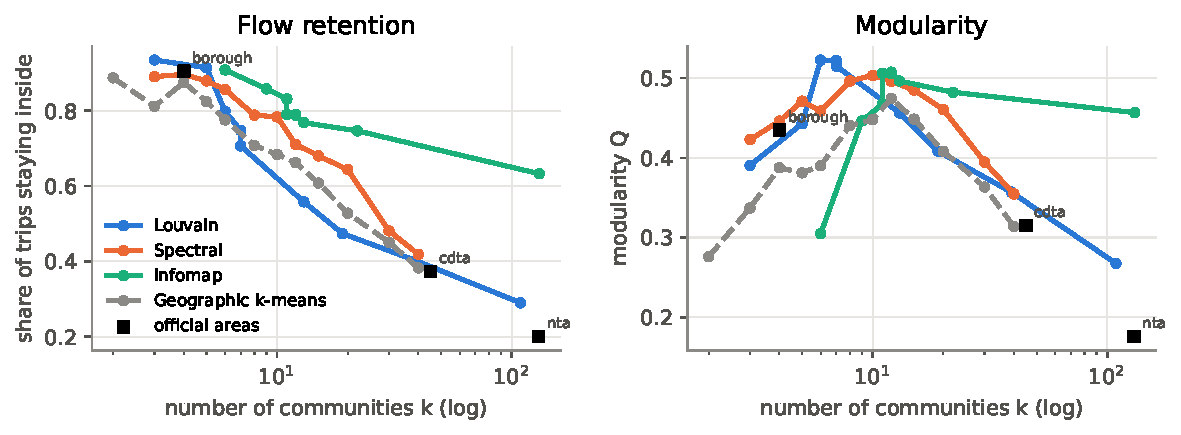
\includegraphics[width=\linewidth]{figures/retention_modularity.pdf}
\caption{Flow retention and modularity against the number of communities. Dashed gray: geographic k-means. Squares: official areas.}\label{fig:ret}
\end{figure}

\textbf{More than geography, but depending on method} (Fig.~\ref{fig:ret}).
Spectral clustering beats the geographic baseline in retention at every $k$ from 3 to 40 (78\% vs 68\% at $k=10$).
Infomap beats it at every $k$ it reaches (79\% vs 66\% at 12 modules; 63\% vs 20\% for 131 modules vs the 130 NTAs).
Louvain beats geography only at low resolution ($k\le6$).
At $\gamma=2$ it is clearly worse (56\% vs 66\% with 13 communities), because high resolution forces it to cut the dense Manhattan core, where trips run in every direction.
On modularity, its own objective, Louvain is highest ($Q=0.52$), with Infomap (0.51) and spectral (0.50) close behind.
All three are well above geography (0.47) and boroughs (0.44).
Boroughs are a very good 4-way split (90.5\% retention, thanks to the rivers), but community districts are no better than geography and NTAs keep only 20\% of trips.
Seed stability separates the methods: Infomap reaches ARI 0.99 (always 12 modules), spectral 0.998, but Louvain only 0.88, and its $k$ varies.

\begin{figure}[t]\centering
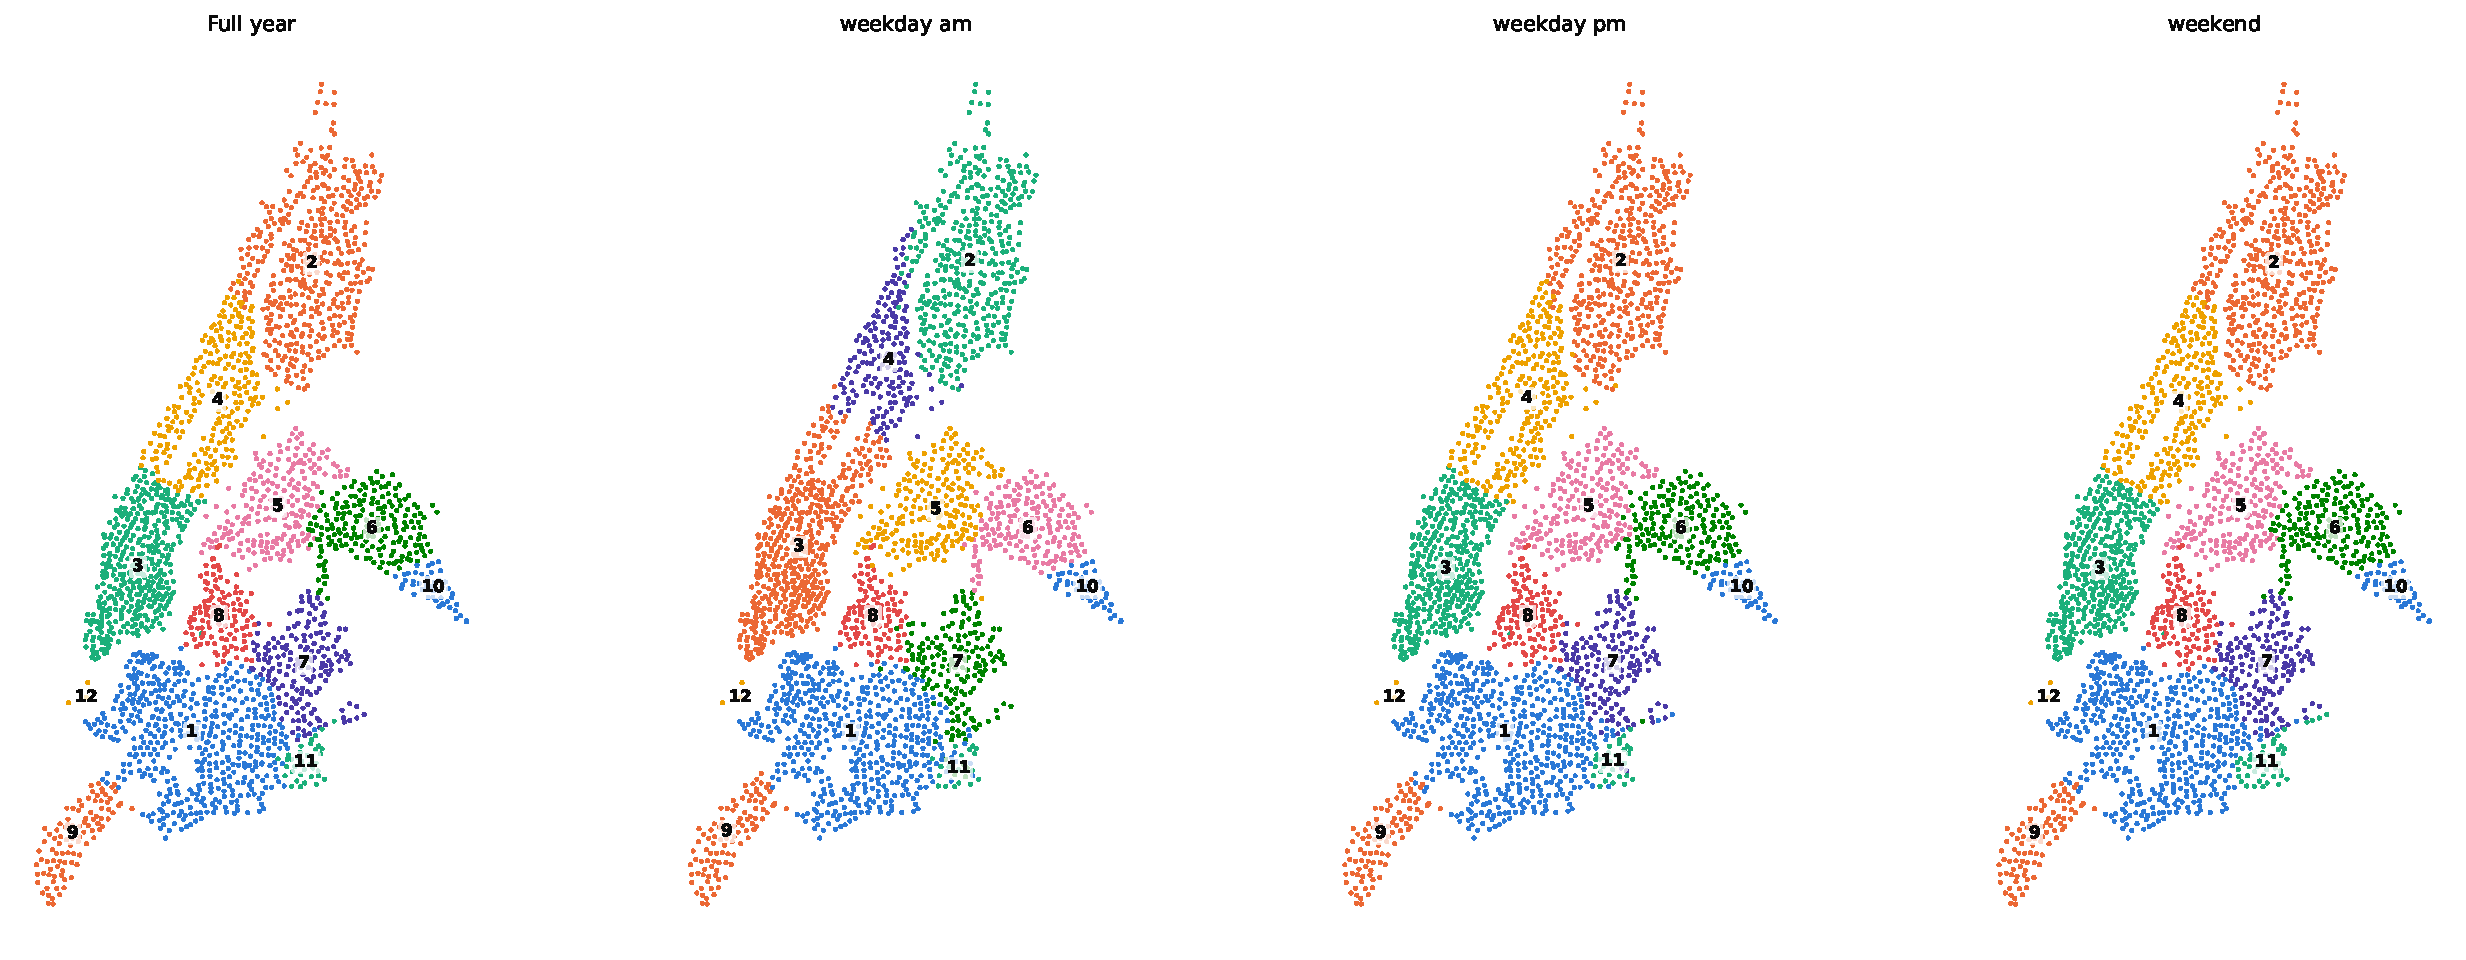
\includegraphics[width=\linewidth]{figures/infomap_slices.pdf}
\caption{Infomap areas for the whole year and three time slices (slice labels matched to the full-year areas by largest overlap).}\label{fig:maps}
\end{figure}

\textbf{The areas} (Fig.~\ref{fig:maps}, full year).
Manhattan south of 59th St forms one area, with 21\,M trips a year starting there and 86\% of them staying inside.
Three areas \emph{cross borough borders}:
northern Manhattan rides with the Bronx (62 Manhattan stations);
Bushwick (Brooklyn) and Ridgewood (Queens) form one area;
and Roosevelt Island (officially Manhattan) belongs with Astoria in Queens.
Governors Island, reachable only by ferry, is its own area (98\% retention), a useful sanity check.

\textbf{Over time.} Each slice's partition is compared with the full-year areas and with its own seed noise.
Nights and weekends do not differ beyond the noise, and midday and the PM rush differ only slightly (ARI 0.90 and 0.97 vs noise levels of 0.96 and 1.00).
The \emph{weekday morning} differs most (ARI 0.87 vs a noise level of 0.99).
Its own partition keeps 84\% of morning trips inside, against 79\% for the full-year areas.
Of its 166 stations that change area, 88 are on the Upper East and West Side, which join the core: the core then reaches 104th St instead of 59th St.

\begin{figure}[t]\centering
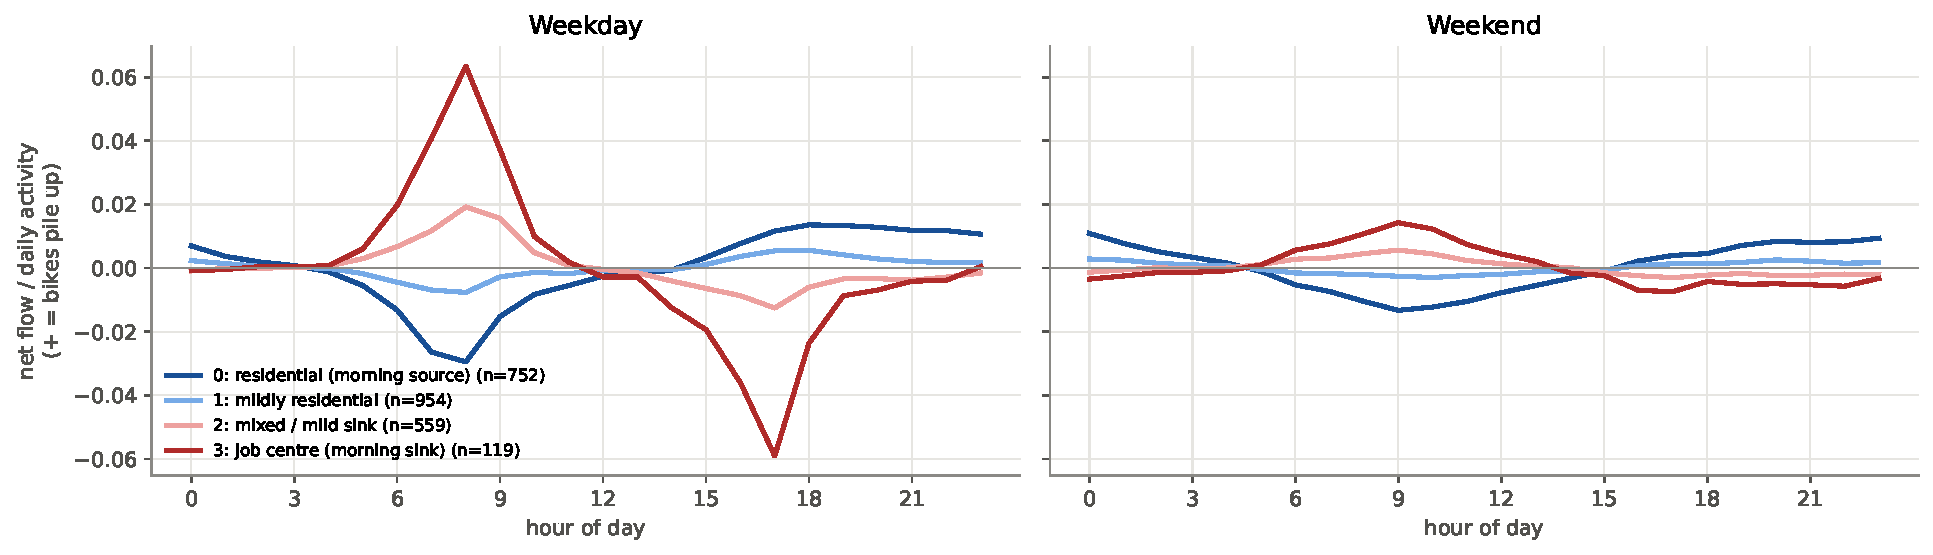
\includegraphics[width=\linewidth]{figures/profile_types.pdf}
\caption{Mean net-flow profiles of the four k-means station types (positive: bikes accumulate).}\label{fig:prof}
\end{figure}

\textbf{Station types} (Fig.~\ref{fig:prof}).
The first principal component explains 37\% of the profile variance (the second only 8\%).
It is a commuting axis, peaking at 8\,am and reversing at 5\,pm, and the stations form a single cloud along it.
Both indices and both algorithms prefer $k=2$ (silhouette 0.25--0.27).
k-means and Ward only partly agree (ARI 0.63 at $k=2$, 0.50 at $k=4$).
We therefore read the $k=4$ types as intervals on one axis.
The 119 ``job-centre'' stations gain about 6\% of their daily trips per hour at 8\,am.
Besides Midtown and FiDi they include Sunset Park West, Long Island City and Downtown Brooklyn, all found without any land-use data.

\textbf{Types within areas.} Every area mixes residential and destination stations.
Only the Manhattan core gains bikes in the weekday morning (+1,660 per day), fed by the Upper East/West Side and Harlem ($-990$) and Brooklyn.
Within Infomap areas, 72\% of the station-level morning imbalance cancels out, but within geographic areas with the same $k$ even more does (78\%).

\section{Evaluation and discussion}
\textbf{What worked.} The flow-based areas pass the test we set up for the ``just geography'' risk.
At equal $k$, Infomap and spectral clustering keep clearly more trips inside than coordinates alone do.
They are reproducible and find known structure without being told: the ferry-only island, the bridge-linked Roosevelt Island, secondary job centres.
The time analysis was only meaningful after measuring seed noise.
Without it, Louvain's run-to-run variation (ARI 0.88) would have looked like differences between time slices.

\textbf{What did not, and why.}
(1) Louvain at high resolution produced areas worse than geography.
We think this is because modularity's null model assumes any two stations could be linked, regardless of distance.
In a dense, well-mixed core a high resolution then makes Louvain cut along arbitrary lines instead of along real flow borders.
(2) Profile clustering found no natural types.
The low silhouette and the weak k-means/Ward agreement show a continuum, which is itself a result: a station's role is a matter of degree.
(3) The Brownsville area keeps only 32\% of its trips and should not be read as a real area.
(4) Retention favours Infomap, since it is close to Infomap's objective, so we also report modularity, on which Infomap comes second.
(5) Self-contained is not the same as balanced.
The trips that cross Infomap borders are mostly one-way morning commutes into the core, so the remaining imbalance gathers at area borders.
For rebalancing, the areas show where riders stay, not where bikes are needed.

\textbf{Limitations.} One year of data, slices by start time only, and a 1-trip-per-day threshold (all stations passed it).
The live station-status feed (GBFS) could show whether shortages stay inside areas.
A collector is implemented but was not run.

\section{Conclusion}
Citi Bike trips define about a dozen functional areas.
They keep more trips inside than geography alone, cross three borough borders, and change mainly in the weekday morning, when the Manhattan core reaches north to 104th St.
Infomap was the most useful method here: it uses trip direction, is stable and matches the question directly.
Station rhythms form a continuum along one commuting axis rather than discrete types.

\section*{Contributions and code}
% TODO: one line per group member
All work (data pipeline, analysis, report): Full Name (s000000).
Code, instructions and notebooks: see the appendix (\texttt{README.md}, \texttt{notebooks/01--03}).
The data are rebuilt from the public sources with \texttt{python -m citibike.download/convert/clean/features/geo}.

\end{document}
